\documentclass{article}
\usepackage[utf8]{inputenc}
\usepackage[top=1.15in, bottom=1.15in, left=1.4in, right=1.4in]{geometry}
\usepackage{graphicx}
\graphicspath{ {images/} }

\begin{document}

\section*{Testes com os Utilizadores}
Neste relatório vão ser apresentados os resultados obtidos após a execução dos testes com utilizadores. Todos os testes foram realizados em condições semelhantes.

\subsection*{Guião}

\subsection*{Caracterização dos Utilizadores}
Os testes foram realizados com 15 utilizadores.
Cerca de 60\% dos utilizadores tinham idades entre os 18 e 25 anos, 6.67\% tem idade inferior a 18, os restantes tinham entre 40 a 50 anos de idade. 40 \% eram do sexo feminino e 60 \% eram estudantes do ensino superior.
Praticamente todos os 15 utilizadores já tinham frequentado bares.

\subsection*{Resultados Tarefa 1}
Nesta tarefa para "medir" a \textbf{eficiência} foi utilizado o número de cliques:
\begin{itemize}
\item\textbf{média:} 4.990;
\item\textbf{desvio-padrão:} 0.765;
\item\textbf{intervalo de confiança:} [4.603, 5.378]; 
\end{itemize}
\begin{figure}[h]
\centering
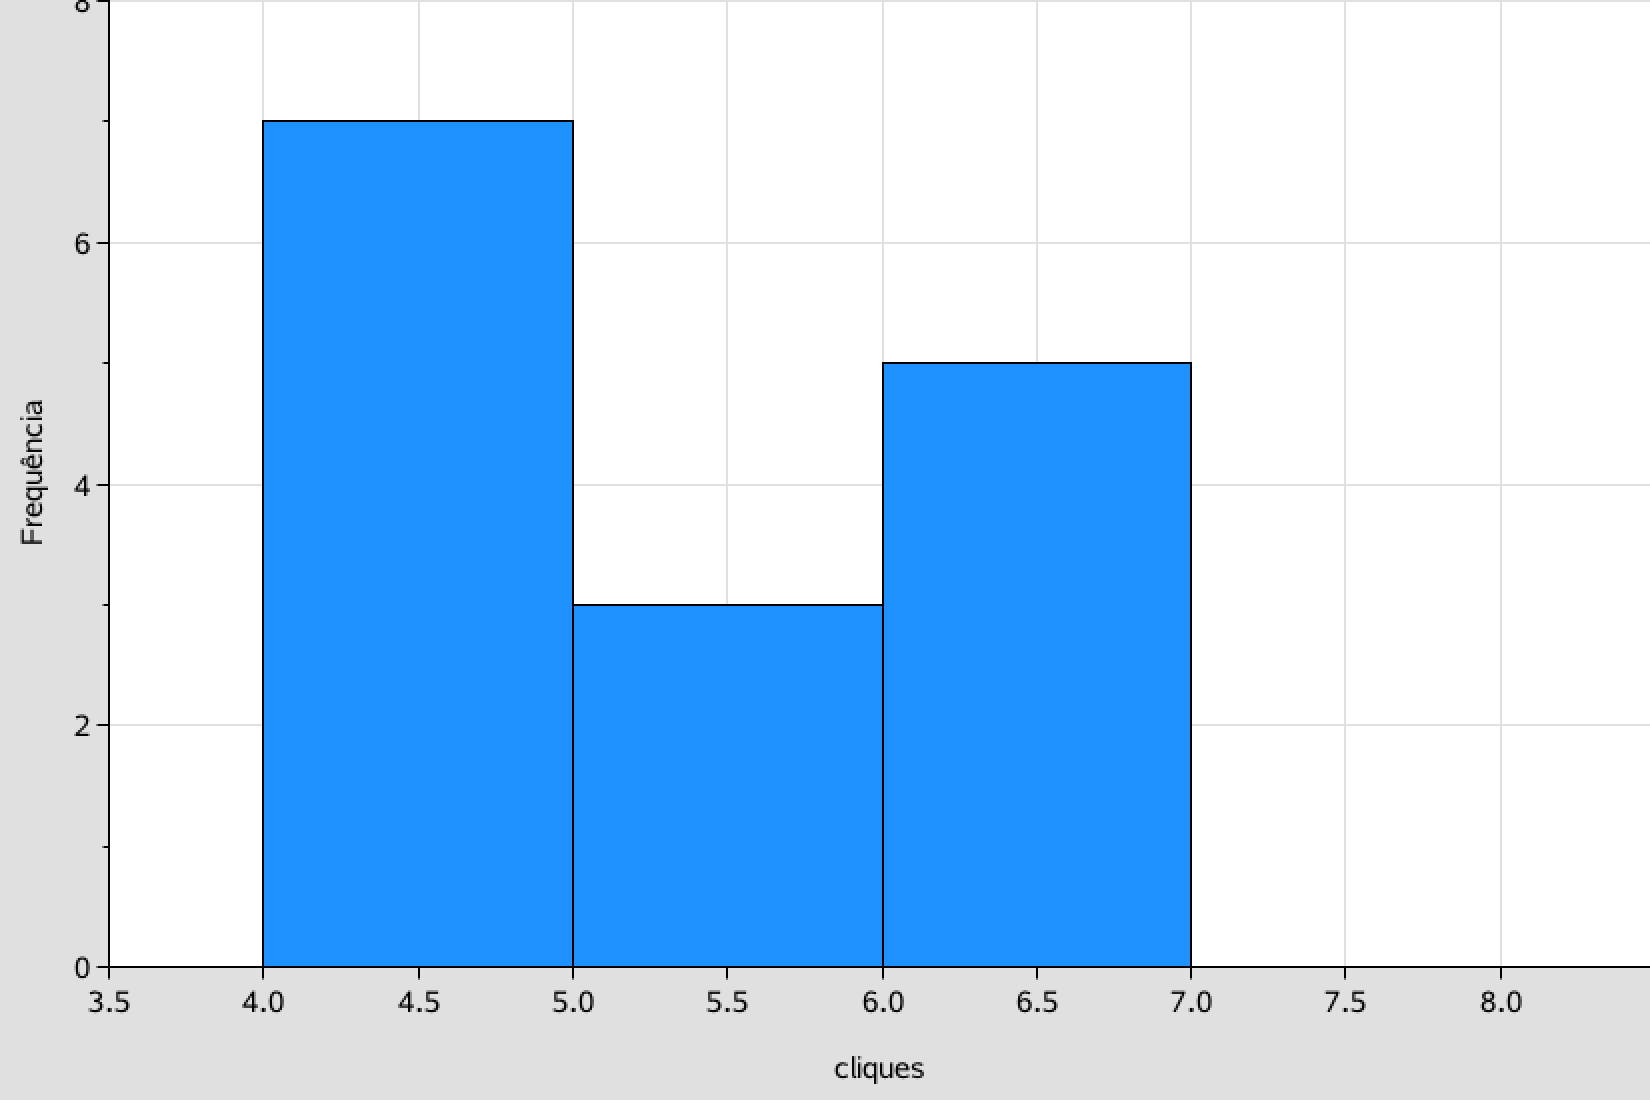
\includegraphics[scale=0.35]{grafico1}
\caption{histograma da frequência do número de cliques na tarefa 1}
\end{figure} Em termos de \textbf{eficácia} nenhum utilizador escolheu a música errada.\\\\
Relativamente à \textbf{satisfação} 93.33\% dos utilizadores Discorda Totalmente com a pergunta feita.\\\\
\textbf{Conclusões:}

Comparando a média de cliques obtida, 4.867, com o valor estipulado, 10, podemos concluir que os utilizadores tiveram mais facilidade na realização da tarefa do que era expectável. Tal deve-se ao facto de a tarefe ter baixa dificuldade e da facilidade dos utilizadores em perceberem a localização dos botões e da música a votar.

 No que diz respeito à eficácia e à satisfação, os resultados obtidos vão ao encontro dos critérios estabelecidos (pelo menos 90\% dos utilizadores escolhe a música correta e em média os utilizadores responderem Não Concorda Totalmente, respetivamente; 

\subsection*{Resultados Tarefa 2}
Nesta tarefa a medida para a \textbf{eficiência} utilizada foram o número de cliques:
\begin{itemize}
\item\textbf{média:} 7.667
\item\textbf{desvio-padrão:} 2.959
\item\textbf{intervalo de confiança:} [6.169, 9.164]
\end{itemize}
\begin{figure}[h]
\centering
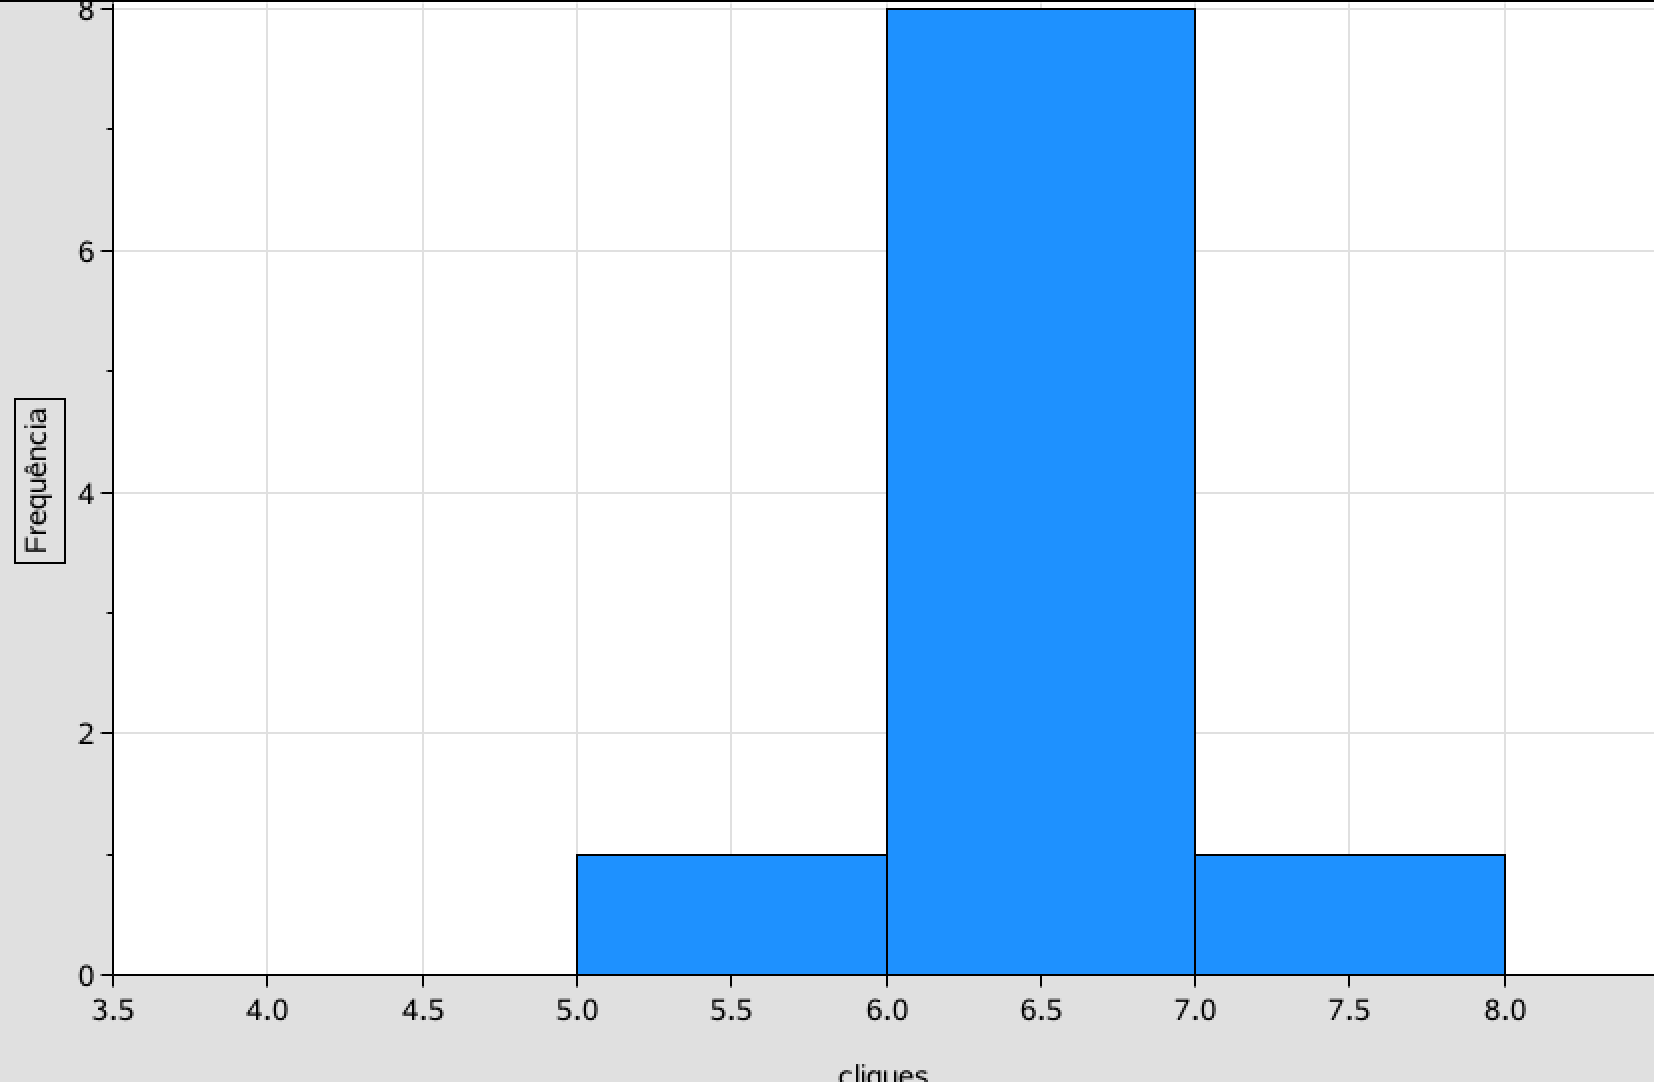
\includegraphics[scale=0.35]{grafico2}
\caption{histograma da frequência do número de cliques na tarefa 2}
\end{figure} Em termos de \textbf{eficácia} foram contados os números de acessos à opção Ajuda:

 - Nenhum utilizador precisou de aceder à opção ajuda logo o valor médio é 0.\\\\
Relativamente à \textbf{satisfação} nenhum utilizador não concordou com a pergunta feita.\\\\
\textbf{Conclusões:}

Tendo em conta o critério de eficiência desta tarefa ( número médio de cliques 9), é possível concluir que a média obtida é inferior ao expectável. Em relação ao critério de eficácia (não mais de 2 acessos à opção ajuda) valor obtido também foi inferior.

No que respeita à satisfação a média das respostas vai ao encontro do que era esperado (não mais de 10\% dos utilizadores responder que Não concorda ou Não concorda totalmente).

No entanto, alguns utilizadores consideram que a opção para Escolher Mesa devia estar mais percetível.

Apesar disso, é possível concluir que os objetivos de usabilidade foram alcançados.

\subsection*{Resultados Tarefa 3}
Nesta tarefa a medida para a \textbf{eficiência} utilizada foi o tempo em segundos:
\begin{itemize}
\item\textbf{média:} 69.333 
\item\textbf{desvio-padrão:} 24.864
\item\textbf{intervalo de confiança:} [56.750, 81.916]
\end{itemize}
\begin{figure}[h]
\centering
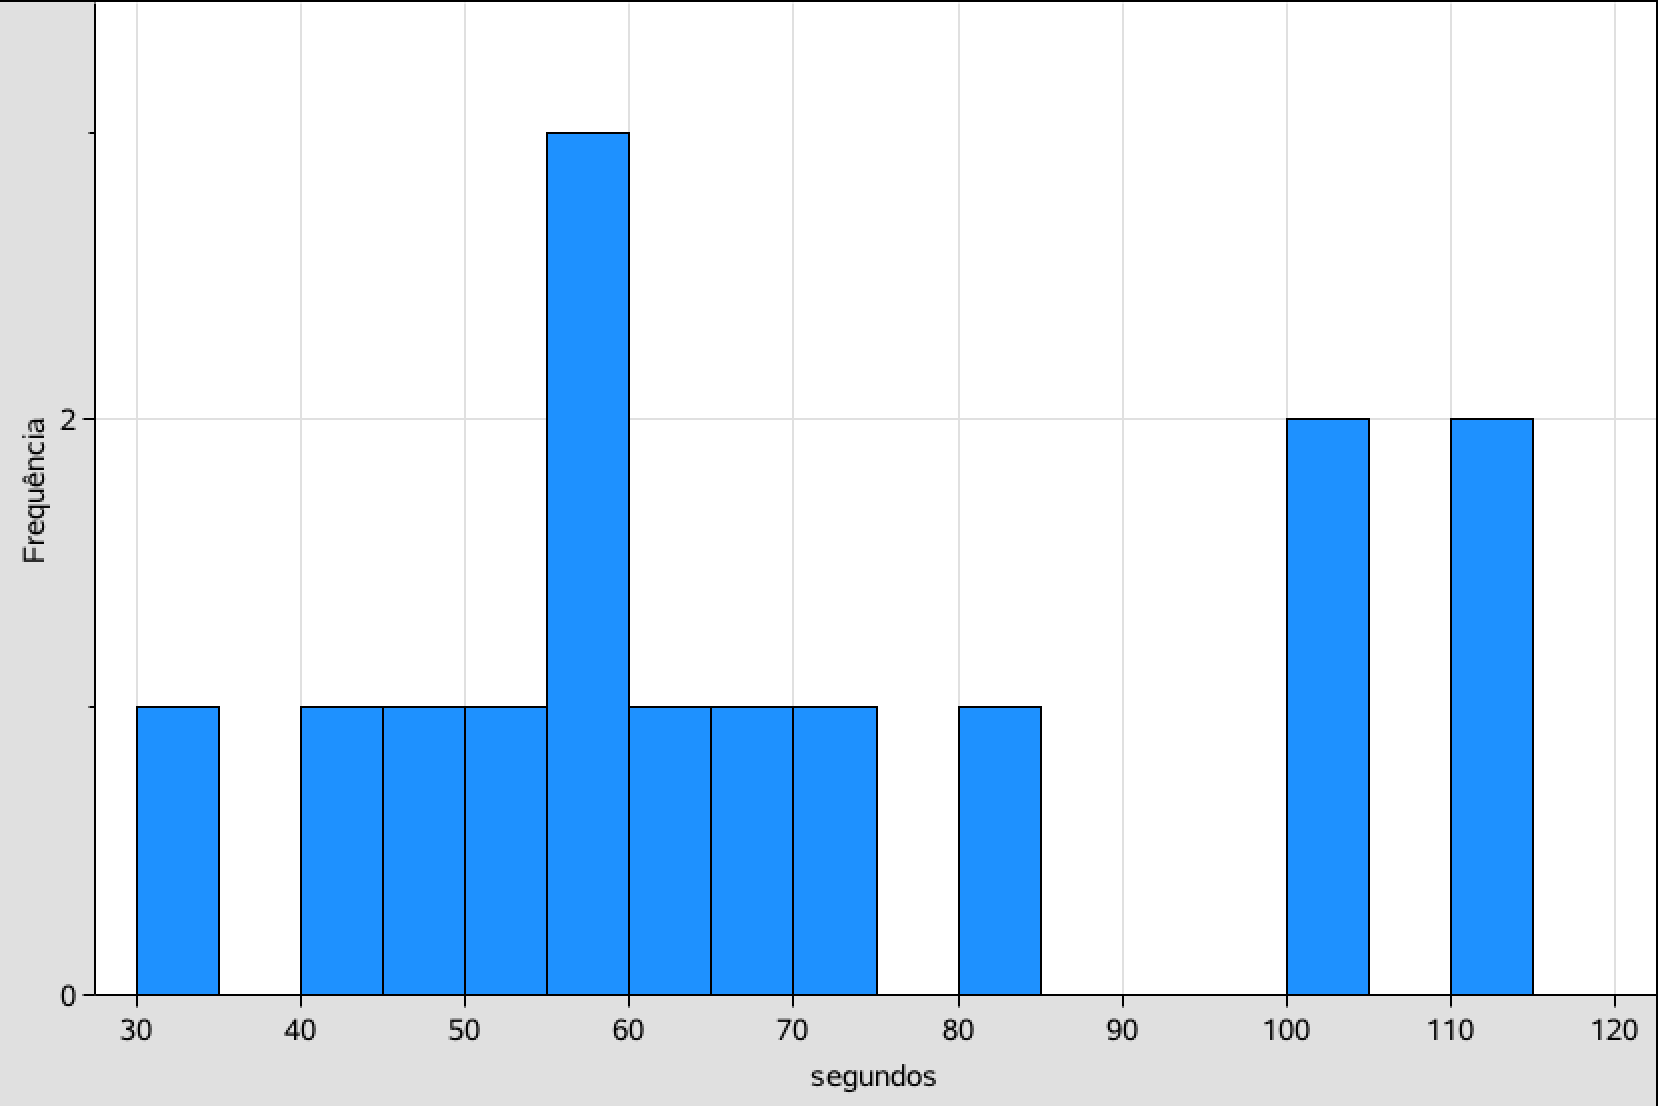
\includegraphics[scale=0.35]{grafico3}
\caption{histograma da frequência do tempo despendido na tarefa 3}
\end{figure} Em termos de \textbf{eficácia}:
 - Apenas 6.67\% dos utilizadores efetuou de forma incorreta o pedido e/ou pagamento \\\\
Relativamente à \textbf{satisfação} cerca de 87\% dos utilizadores Concordou parcialmente ou totalmente com a questão.\\\\
\textbf{Conclusões:}

Comparando o tempo médio estipulado no relatório anterior para realizar a tarefa, 1 minuto, podemos verificar que o valor obtido após a realização dos testes é ligeiramente superior. Tal deve-se ao facto de no pagamento as setas para transitar os itens de um retângulo para o outro não serem percetíveis o suficiente.

No entanto, os resultados obtidos relativos à eficácia e à satisfação vão de encontro com os seus critérios (não mais que 15\% dos utilizadores concretizaram o pedido e/ou pagamento de forma incorreta e pelo menos 80\% dos utilizadores responde Concordo ou Concordo totalmente, respetivamente).

Logo, o único objetivo de usabilidade que não foi atingido foi o de eficiência.

\end{document}